\section{Experiment}
\label{experiment}
In this section, we conduct extensive experiments on different datasets which
contain the semantic measurement by human perceptions. We compute the Pearson
correlation coefficient $\gamma$, Spearman correlation coefficient $\rho$ and
harmonic mean coefficient $\mu=\frac{2\gamma\rho}{\gamma+\rho}$
between results of experiments and scores of human judgement to evaluate the performance of our model. 
% The model is implemented on cpu Core-7-7700K@4.20GHz$\times$8 machine with 16GB memory and ArchLinux platform.

\subsection{Dataset}
The knowledge association network $KAN_{wiki}$ is conducted based on the Wikipedia\footnote{https://dumps.wikimedia.your.org/}
and DBPedia\footnote{https://wiki.dbpedia.org/downloads-2016-10}. The details about the basic dataset are shown in table
\ref{basicdataset}. You will find the number of entities is larger than documents in Wikipedia, since the entities set
contain entities extracted not only from Wikipedia but also some other semantic dataset such as ontololy language, YAGO and
so on. It is necessary to preprocess the Wikipedia before constructing network $KAN_{wiki}$. As shown in figure \ref{overview},
for each page in Wikipedia, we remove the stop words and punctuation, ignore the shorter pages whose words number less than 50, and
ignore some special namespaces such as \emph{Category, File, Template} and so on.

\renewcommand\arraystretch{1.2}
\begin{table}[H]
    \center
    \begin{tabular}{|p{1.6cm}|p{1.6cm}|p{1.6cm}|p{1.6cm}|}
    \hline
              & Documents & Date        \\ \hline
    Wikipedia & 5.5M      & 2016-10     \\ \hline
    DBPedia   & 6.6M      & 2016-10     \\ \hline
              & Entities   & Date \\ \hline
    \end{tabular}
    \caption{Wikipedia and DBpedia Information}
    \label{basicdataset}
\end{table}

\subsection{Evaluation}
A great number of datasets record the scores of human quantitative judgement
for semantic relatedness. We evaluate $KAN_{wiki}$ on three frequently used datasets that
are listed in table \ref{basicdataset}.
Based on the standard dataset, we compare our model to other existing models, such as
ESA\cite{ijcai/GabrilovichM07}, SSA\cite{aaai/HassanM11}, word2vec\cite{corr/Mikolov13},
SaSA\cite{aaai/WuG15}, AN\cite{aaai/ZhangZH15} and HAN\cite{aaai/GongXH18}.

\renewcommand\arraystretch{1.2}
\begin{table}
    \center
    \begin{tabular}{|p{1cm}|p{0.7cm}|p{0.7cm}|p{4.2cm}|}
    \hline
    dataset   & word pairs & score scope & reference \\ \hline
    MC        & 30         & [0,4]       & Miller\&Charles1991          \\ \hline 
    RG        & 65         & [0,4]       & Rubenstein\&Goodenough1965       \\ \hline
    WS353     & 353        & [0,10]      & Finkelstein et al.2002         \\ \hline
    \end{tabular}
    \caption{Wikipedia and DBpedia Information}
    \label{basicdataset}
\end{table}

\renewcommand\arraystretch{1.3}
\begin{table*}
    \center
    \begin{tabular}{l|c|c|c|c|c|c|c|c|c}
    \hline
    \multirow{2}{*}{Model} & \multicolumn{3}{c|}{$\lambda$}     & \multicolumn{3}{c|}{$\rho$}          & \multicolumn{3}{c}{$\mu$} \\ \cline{2-10} 
                           & \textbf{MC}&\textbf{RG}&\textbf{MS353} & \textbf{MC}&\textbf{RG}&\textbf{MS353} & \textbf{MC}&\textbf{RG}&\textbf{MS353}\\ \hline
    ESA                    & 0.588 &  - -  & 0.503 & 0.727 &  - -   & 0.748 & 0.650 &  - -   & 0.602   \\ \hline
    SSA                    & 0.879 & 0.861 & 0.590 & 0.843 & 0.833 & 0.604 & 0.861 & 0.847 & 0.597   \\ \hline
    word2vec               & 0.852 & 0.834 & 0.633 & 0.836 & 0.812 & 0.645 & 0.844 & 0.823 & 0.639   \\ \hline
    SaSA                   & 0.886 & 0.882 & 0.733 & 0.855 & 0.851 & 0.739 & 0.870 & 0.866 & 0.736   \\ \hline
    $AN_{wiki}$            & 0.865 & 0.858 & 0.740 & 0.848 & 0.843 & 0.813 & 0.856 & 0.850 & 0.775   \\ \hline
    $HAN_{wiki}$           & 0.886 & 0.884 & 0.772 & 0.860 & 0.857 & 0.826 & 0.873 & 0.870 & 0.798   \\ \hline
    $KAN_{cnt}$       & 0.850 & 0.826 & 0.630 & 0.836 & 0.805 & 0.633 & 0.842 & 0.816 & 0.631   \\ \hline
    $KAN_{tf\_idf}$         & \textbf{0.892} & \textbf{0.887} & \textbf{0.789} & \textbf{0.872} & \textbf{0.865} & \textbf{0.841} & \textbf{0.882} & \textbf{0.876} & \textbf{0.814} \\ \hline
    \end{tabular}
    \caption{Pearson-$\lambda$, Spearman-$\rho$, harmonic mean-$\mu$ on the word relatedness datasets}
    \label{srresult}
\end{table*}


\subsubsection{Parameters tuning}
In this paper, it is necessary to determine the following parameters:
\begin{itemize}
\item Recall word-to-word, we train word2vec in Wikipedia to get the vector representations for words.
And we adopt \emph{100 dimension, 30 window size, Skip-gram model and negative sampling} for word2vec
following \emph{KAN}. 

\item In the section of attributes embedding, we set \emph{margin $\ell=0.05$, dimentsion $d=100$, negative sampling number $k=50$} for 
attributes graph embedding, and we set the learning rate of SGD as $0.1$ to optimize the margin ranking loss.

\item In the section of embedding for topological structure, the parameters $p$ and $q$ control the search bias $\mathrm{a}$.
The Skip-gram model is used for training the sequences of random walk, and we set the \emph{100 dimension, 10 window size} 
as the basic parameters in Skip-gram model.

\item $\alpha$ is proposed for the balance of attributes information and topological structure. $\varphi$ trades off the weight
of word-layer against concept-layer.
\end{itemize}

\begin{figure}
    \flushleft
    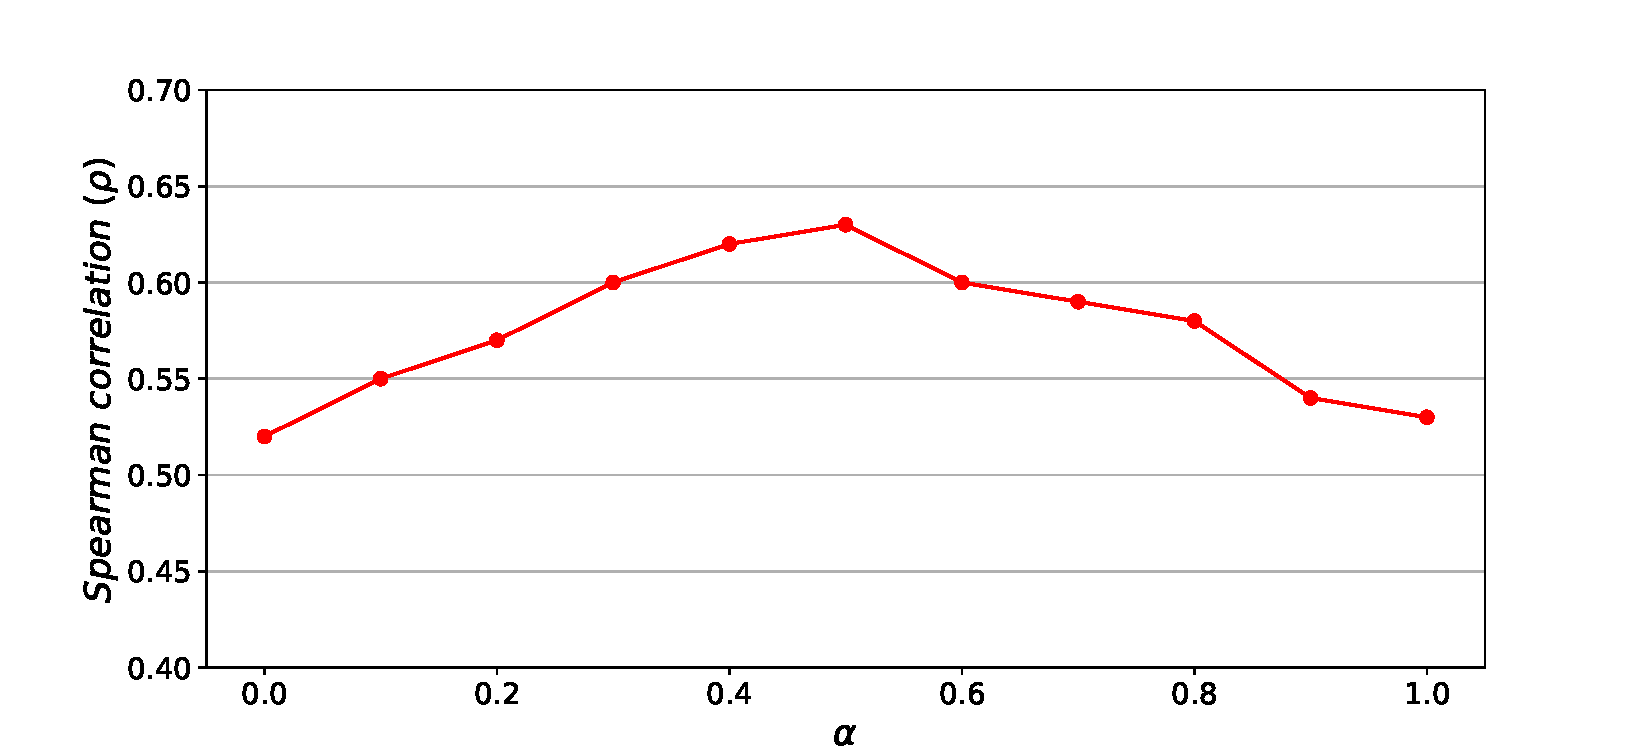
\includegraphics[width=0.5\textwidth]{pic/params_alpha.pdf}\\
    \caption{$\alpha$ tuning on WS-Rel only consider entity-to-entity layer}
    \label{alpha}
\end{figure}

In order to get the optimal correlation, we pick \emph{WS-Rel}\cite{ws/AgirreAHKPS09} to tune the $p$, $q$ and $\alpha$.
since there are not many comparison systems in the literature that report results on this dataset.
This dataset contains 252 pairs of words along with relatedness judgement.
We compute word semantic relatedness just on entity-to-entity layer($f_e$) and find the optimal values
$p=3$ and $q=1$ respectively. As for $\alpha$, as shown in figure \ref{alpha}, Spearman correlation($\rho$) increases evidently
when the importance of topological structure is raised. And we get the optimal values for $\alpha$ to be $0.5$,
which means attributes information and topological structure play the same role for semantic relatedness measurement.


\begin{figure}
    \flushleft
    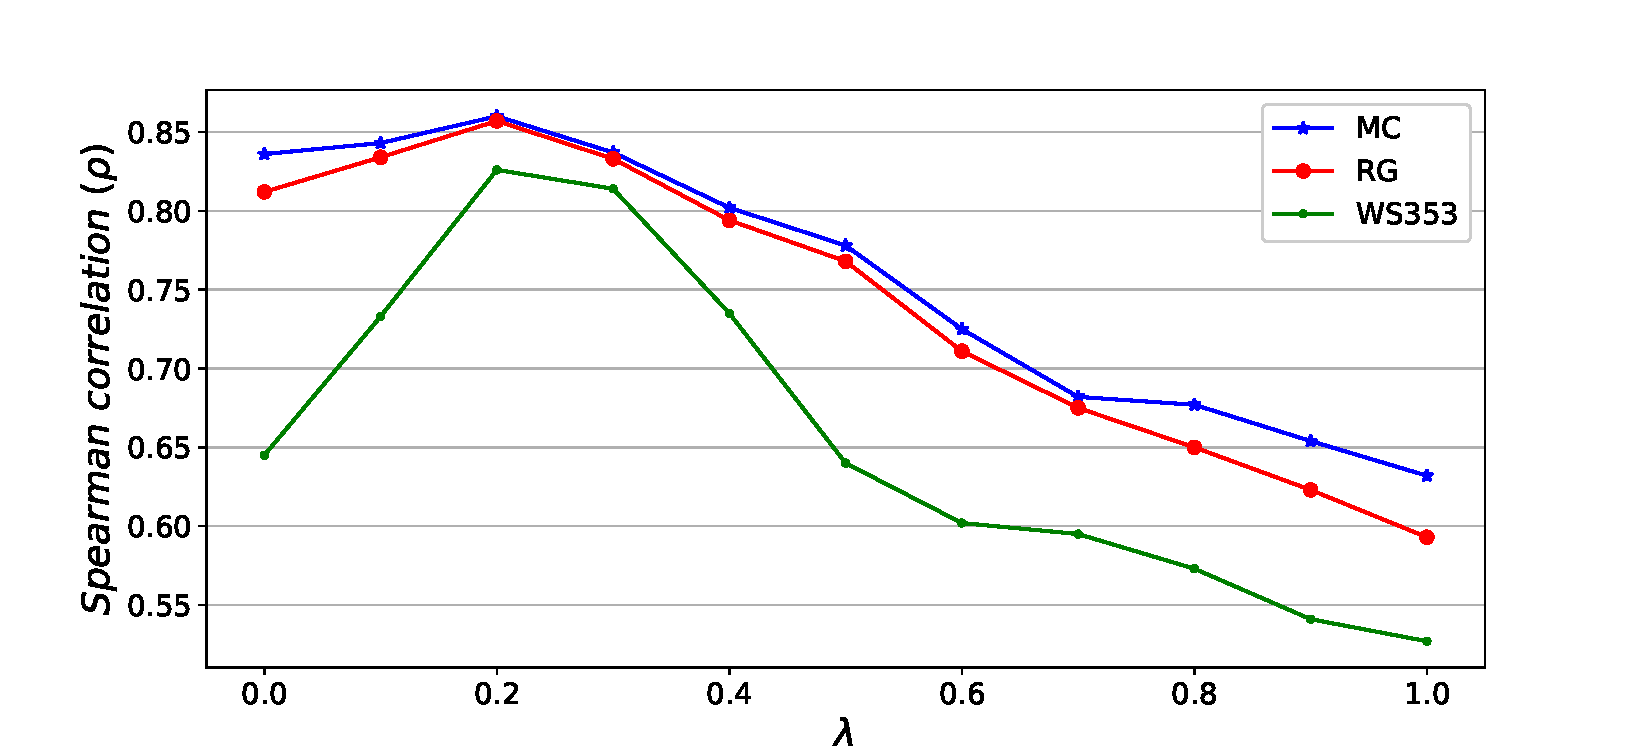
\includegraphics[width=0.5\textwidth]{pic/params_lambda.pdf}\\
    \caption{Performance with value of $\lambda$}
    \label{lambda}
\end{figure}


Another parameter $\varphi$ trades off the weight of word-layer
relatedness $F_w$ against concept-layer relatedness $F_c$. We set tuning rate of $\varphi$
is 0.1. Figure \ref{lambda} shows the results w.r.t the multiple value of $\varphi$ on $KAN_{tf\_idf}$, and when
$\varphi=0.2$, we get the largest Spearman correlation($\rho$). Obviously, $F_w$ have a leading role and
our $F_c$ make a great supplement for final semantic relatedness measurement.

\subsubsection{Comparions results}

Evaluation result of word semantic relatedness on different correlation coefficient is shown in table \ref{srresult}.
Recall embedding for topological structure of our network, there are two strategies to weight the relationship among
entities: 1) $W_{cnt}(e_i, e_j)$ denote the co-occurrence frequence of $e_j$ in page of $e_i$; 2) $W_{tf\_idf}(e_i, e_j)$
adopt $tf\_idf$ to judge how import an entity is to the other. Based on these two weight strategies, we construct $KAN_{cnt}$
and $KAN_{tf\_idf}$ respectively.
We can see that the $KAN_{tf\_idf}$ outperforms $KAN_{cnt}$ in different datasets and measurement coefficients,
since $tf\_idf$ increases proportionally the number of times a term($t$) appears in the page of an entity.
And the value of tf-idf is offset by the number of pages in Wikipedia that contain the item $t$, which helps
to adjust the weight for the fact that some items appear more frequently in general.

When compared with other methods shown in table \ref{srresult}, our method performs better.
$AN_{wiki}$ and $KAN_{wiki}$ get excellent performance on word semantic relatedness on the idea of \emph{free association network},
which improve the weakness of co-occurrence-based methods. $KAN_{tf\_idf}$ measure semantic relatedness
among concepts on the shoulder of $AN_{wiki}$ and $KAN_{wiki}$. We adopt two different model to
capture the semantic of attributes($G_{attr}$) and topological structure($G_t$) in $KAN_{tf\_idf}$ and make the
model more flexible and expressive.